\chapter{Info utili}

\begin{figure}[H]
    \centering
    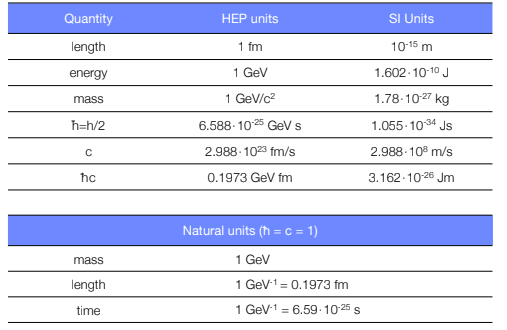
\includegraphics[width=0.8\textwidth]{./Chapters/images/Appendice/image-20220214164823650.png}
    \caption{Unità di misure usate in fisica delle alte energie}
    \label{fig:}
\end{figure}

% TODO Aggiungi massa particelle più importanti

% TODO Aggiungi dati su materiali più importanti

% TODO Aggiungi info utili da pdg man mano che fai esercizi

\begin{itemize}
    \item Sorgenti radioattive più usate: \url{https://pdg.lbl.gov/2018/reviews/rpp2018-rev-commonly-used-radioactive-sources.pdf}
    \item Proprietà di alcuni elementi, Stopping power e range per muoni  e lunghezze di assorbimento adroniche per pioni : \url{https://pdg.lbl.gov/2020/AtomicNuclearProperties/index.html} 
    \item NIST stopping powers for electrons and positrons in arbitrary materials: \url{http://physics.nist.gov/PhysRefData/Star/Text/ESTAR.html}
    \item NIST stopping power and range tables for protons in selected materials: \url{http://physics.nist.gov/PhysRefData/Star/Text/PSTAR.html}
    \item NIST stopping power and range tables for alpha particles in selected materials: \url{physics.nist.gov/PhysRefData/Star/Text/ASTAR.html}
\end{itemize}




